\documentclass{simpledoc}


\newcommand{\soft}{\textsc{FindGrains} }
\newcommand{\var}[1]{\color{myblue}$\langle$#1$\rangle$}
\newcommand{\opt}[1]{\color{myblue}$[$#1$]$}
\newcommand{\file}[1]{\textit{\color{myblue}#1}}
\newcommand{\screen}[1]{\texttt{\color{myblue}#1}}
\newcommand{\scr}[1]{\texttt{\color{myblue}#1}}
\newcommand{\key}[1]{\fbox{\color{myblue}#1}}

\title{\textsc{FindGrains} -- Documentation}
\author{
\textbf{Vincent Richefeu} $\langle$Vincent.Richefeu@3sr-grenoble.fr$\rangle$\\
Lab. 3SR, University of Grenoble, France
}

\pagestyle{myfootings}
\markboth{FindGrains, user guide}%
         {FindGrains, user guide}

%%%%%%%%%%%%%%%%%%%%%%%%%%%%%%%%%%%
%%%%%%%%%%%%%%%%%%%%%%%%%%%%%%%%%%%
\begin{document}

\maketitle

\begin{abstract}
This document describes how to use the code \soft to find the initial positions and radii of circular grains from a \textsc{Tiff} image. This data is used as input in the code \textsc{Tracker} when working with the $1\gamma 2 \varepsilon$ device.
\end{abstract}

\tableofcontents

\newpage

\section{Introduction}

\soft is a soft developed to find the initial positions and radii of circular grains from a \textsc{Tiff} image. 
 It is written with C++ language and should easily be compiled on any operating system (linux, Windows or Mac OS X).
\soft\! requires the library \screen{libtiff} to read \textsc{Tiff} images, and may be compiled with OpenMP. 

\attention
{\color{red} This code is \textit{not} free. It is designed for academic researches only.}

\section{Compilation}

To compile \soft, the following command should make the job on an Unix-like OS:
%
\begin{verbatim}
$ g++ -O3 -fopenmp FindGrains.cpp -o FindGrains -ltiff
\end{verbatim}
%
However, on Mac OS X, you may install \scr{gcc-5} (or more recent) using \scr{Homebrew} for example. 

\section{Procedure}

To run the procedure of finding grains, a command file is invoked that way:
%
\begin{verbatim}
$ ./FindGrains CommandeFile.txt
\end{verbatim}
%
where an example of CommandeFile.txt could be:
\begin{verbatim}
! The path to the image file (without spaces)
image_name JCISD1_13-06-14_0015.tif

! Minimum and maximum radii in pixel-units
Rmin  14
Rmax  168

! Number of smothing passes
nsmooth  2

! Coordinates of the four corners
zone.xTL  578
zone.yTL  1453
zone.xTR  7260
zone.yTR  1510
zone.xBR  7255
zone.yBR  7070
zone.xBL  568
zone.yBL  7043

! Radius of the rounded parts in the corners of 1g2e frame
zone.Rcorners  231

! Gray level threshold for the segmentation.
threshold  14000
\end{verbatim}
%
All the parameters speak by themselves and can be found by using \scr{imagej} for example.
We will now follow, step by step, how to use \soft.

The application has been developed specifically for the tracking of circular grains in $1\gamma 2 \varepsilon$ photographs. We need to start with the first photograph of the sample that will be use as reference in the tracking procedure.
Notice that it is required that this photograph is a \textsc{Tiff} 16-bits image, like that one:
%
\begin{center}
  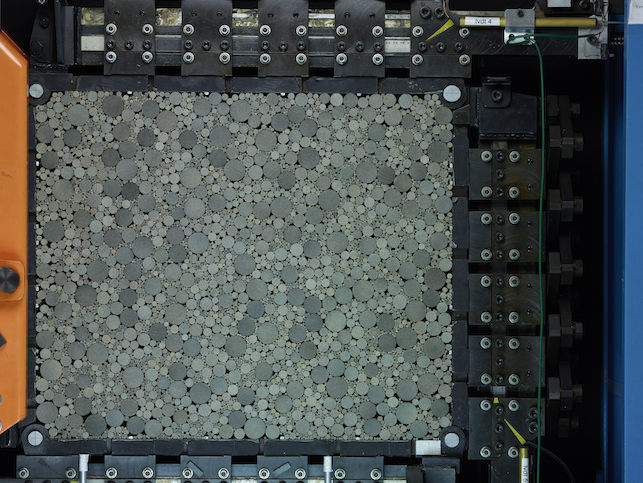
\includegraphics[width=0.7\textwidth]{SampleImage.png} 
\end{center}

The first step of the procedure aims to mask the zone outside the sample, and to make a histogram of gray levels (only in the sample zone). This histogram is needed to define the threshold value that is used to perform a segmentation.
The sample zone is defined by the four corner positions and the radius of these corners. The procedure to find them by using \scr{imagej} is not described here. When running the application with \scr{threshold 0} (in the command file), a histogram will be generated in the file \scr{histo.txt} and \soft\ will end. The histogram may be like that one:
%
\begin{center}
  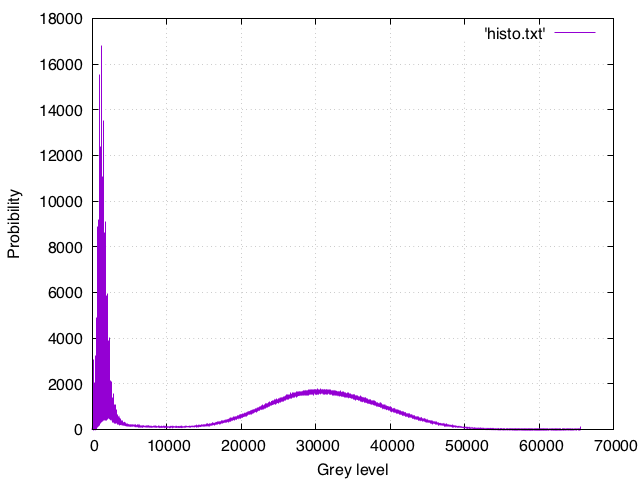
\includegraphics[width=0.7\textwidth]{histo.png} 
\end{center}
%
where we can see high frequencies of black colors (on the left) and a smaller peak that should correspond to the gray levels of the patterns of the grains. The threshold value can thus be set to the lower grey value of this peak. Here we've got \scr{threshold 14000}.

The second step of the procedure is to run a second time the application, with a non-zero value of the threshold this time. The sequence of processing will be as follows:
%
\begin{itemize}
\item Mask the outside of the sample 
\begin{center}
  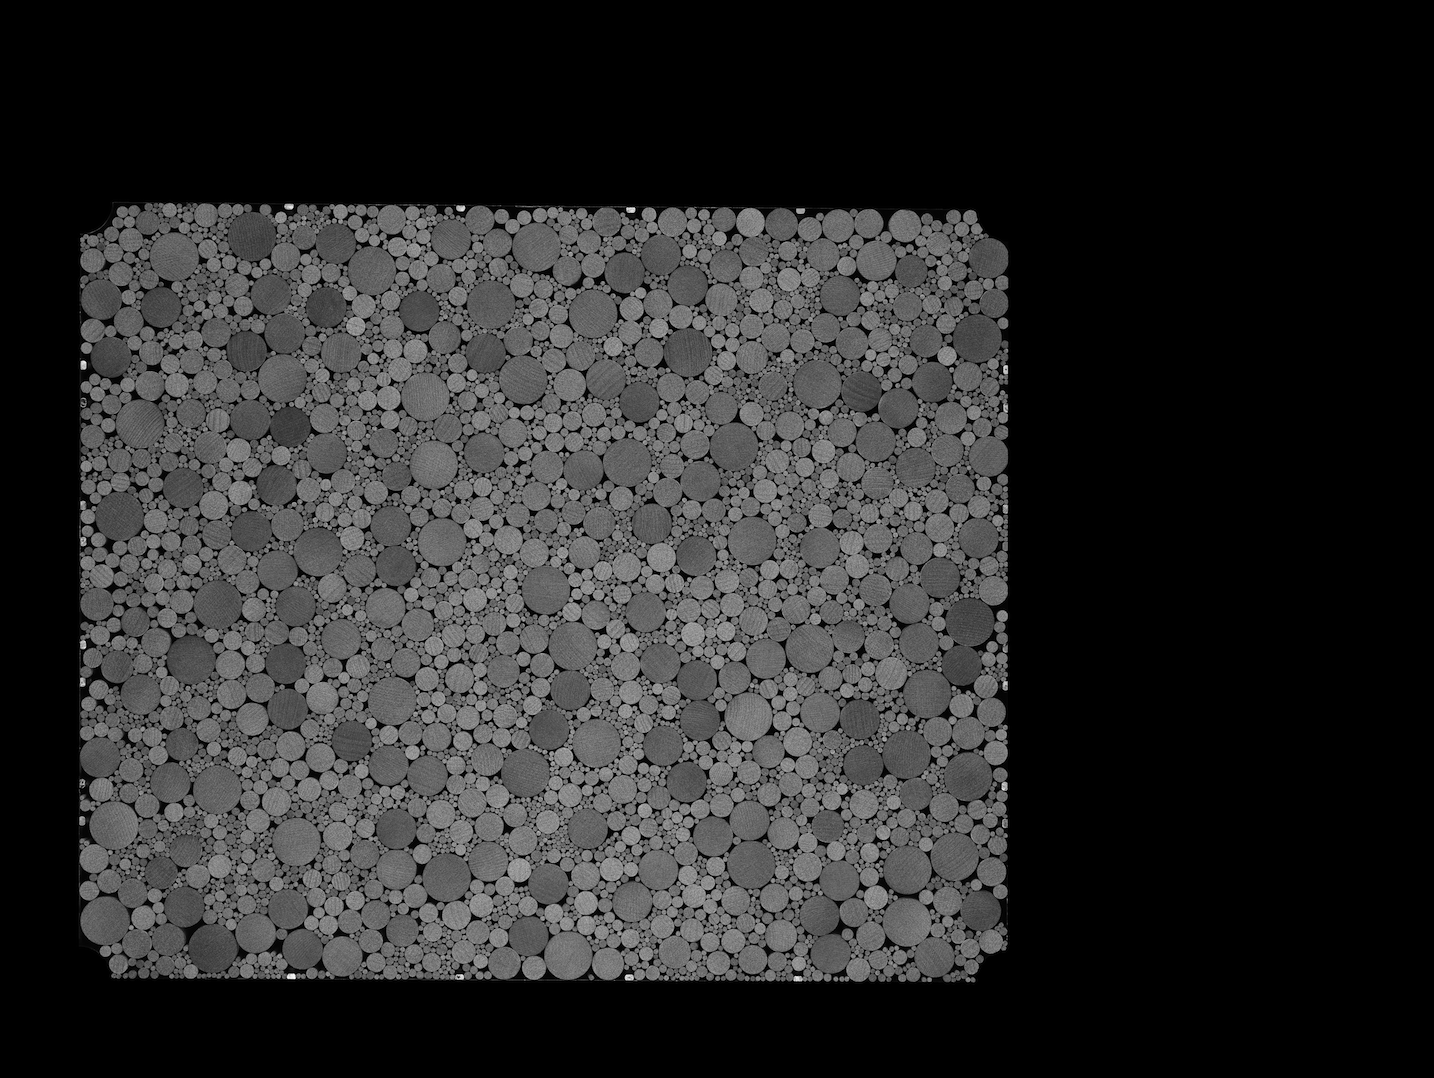
\includegraphics[width=0.7\textwidth]{zoning.png} 
\end{center}
\item Apply a smoothing filter many times (the number of passes is defined by \scr{nsmooth}) to ease the segmentation that follows.
\item Segment the image so that the grains are white and the voids are black.
\begin{center}
  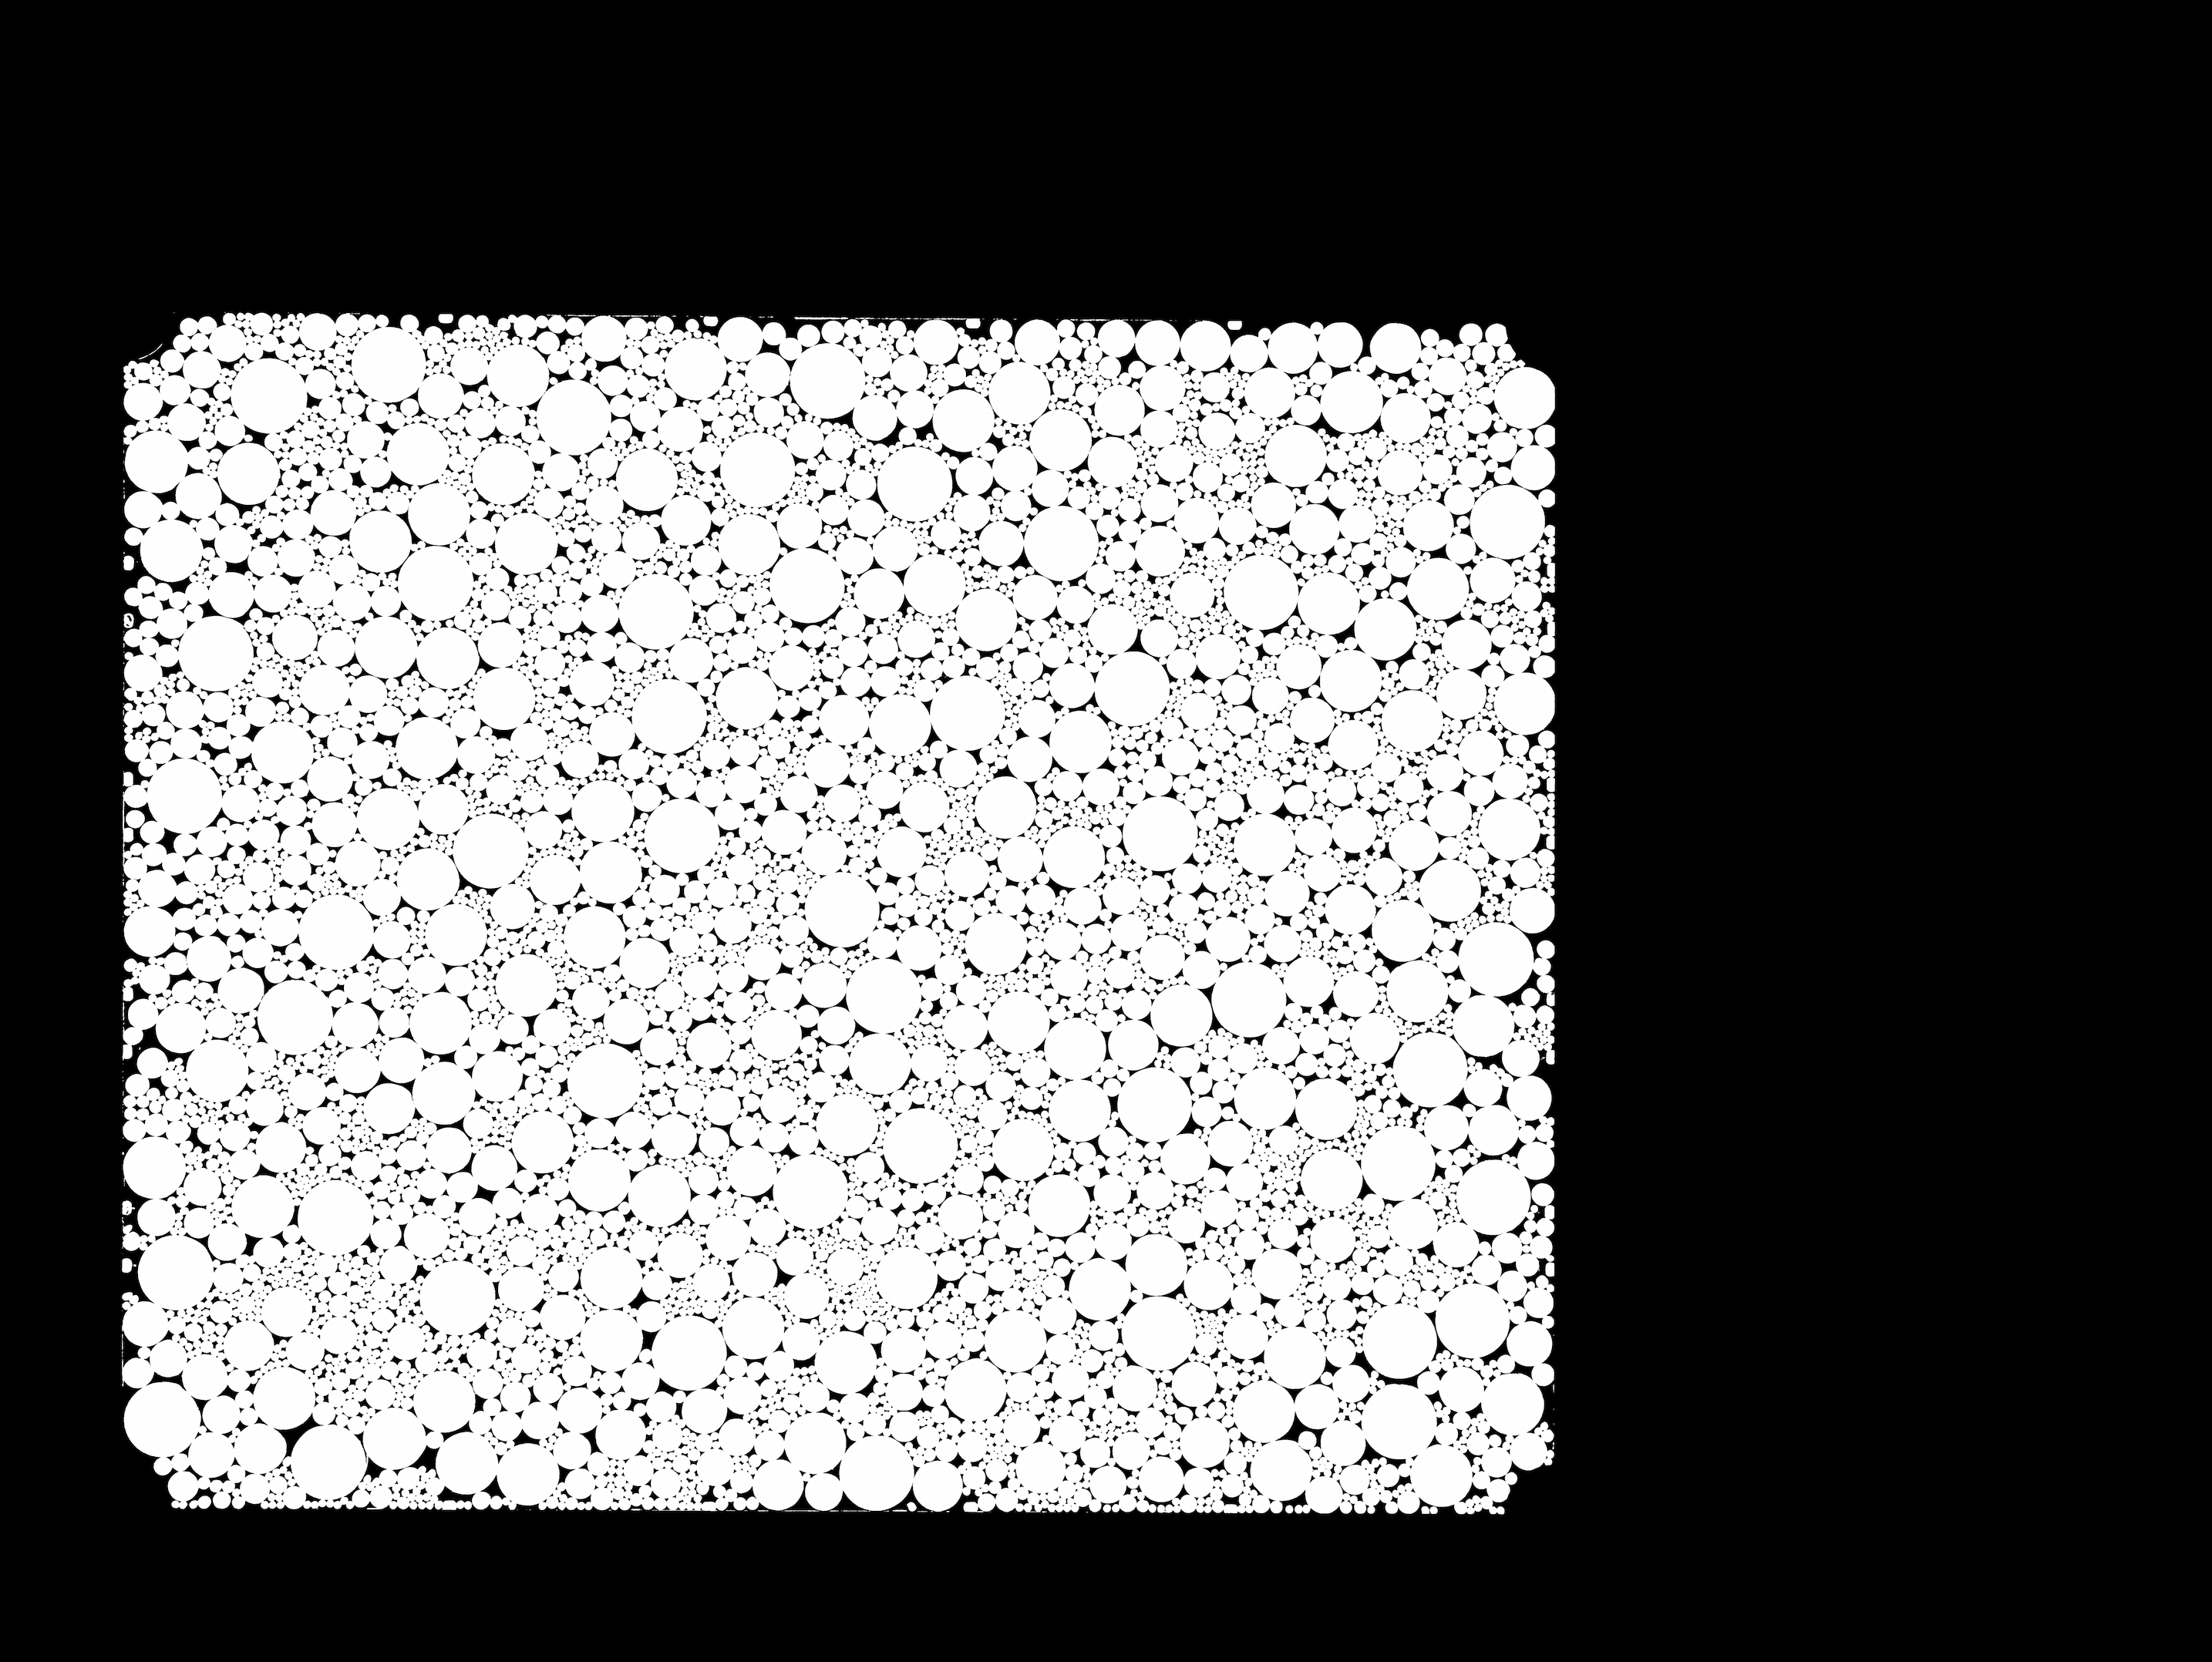
\includegraphics[width=0.7\textwidth]{segment.png} 
\end{center}
\item Compute the distance of each white pixel with the closest black pixel (this step is the longest. It is thus parallelized by means of OpenMP).
\begin{center}
  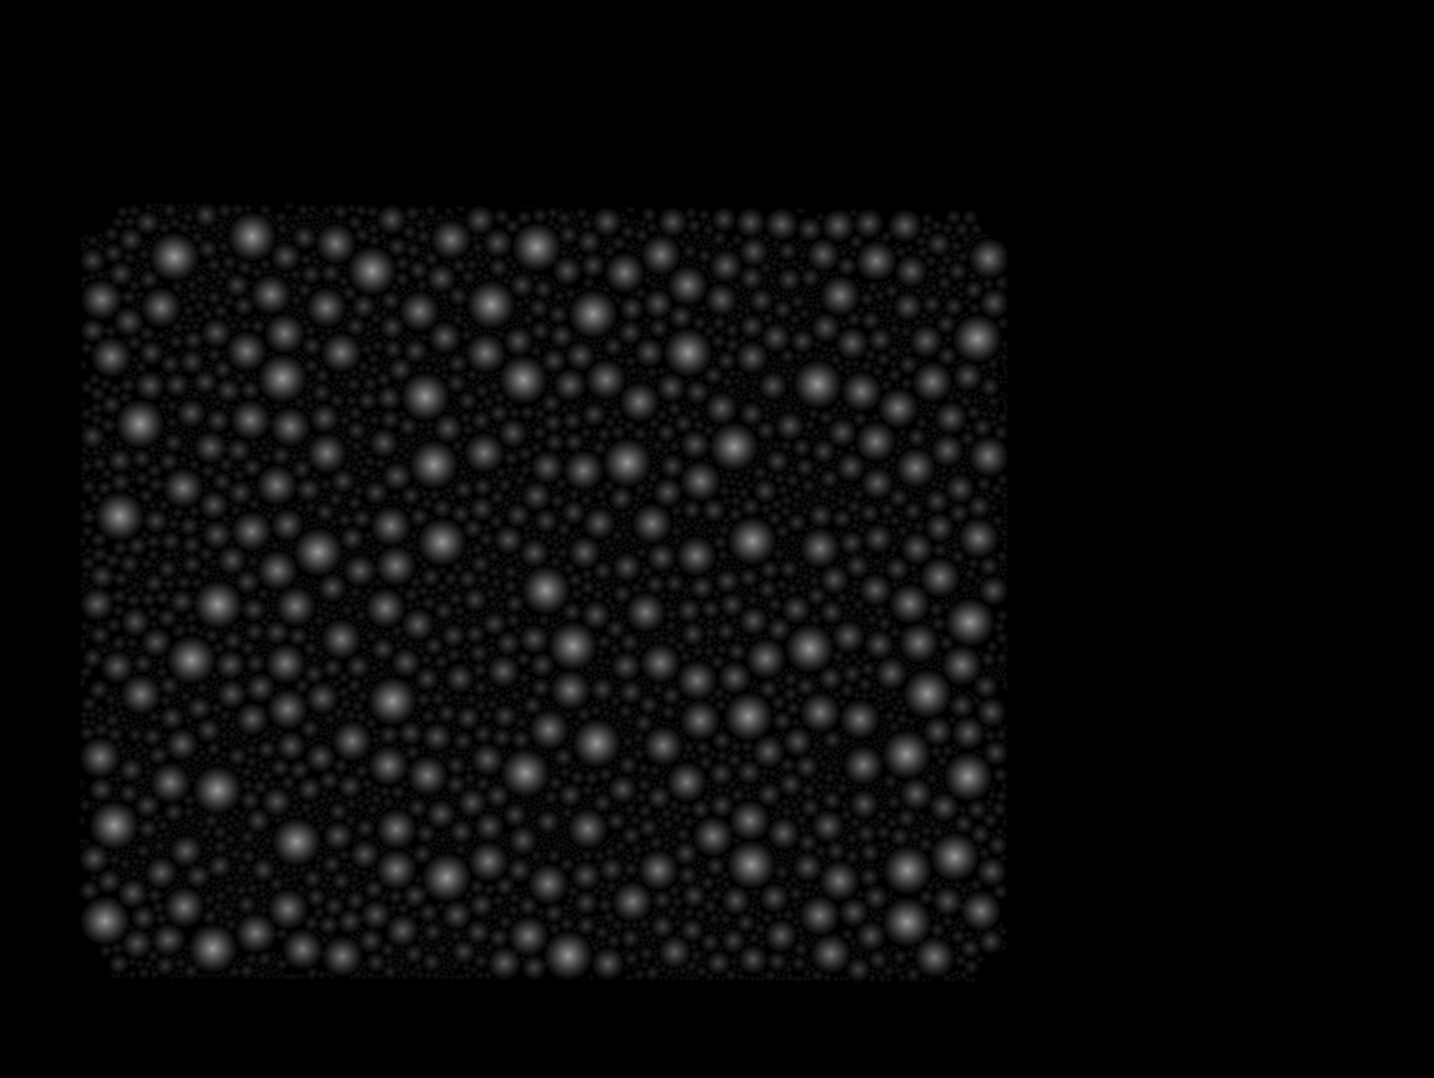
\includegraphics[width=0.7\textwidth]{distance.png} 
\end{center}
\item Extract the positions and radii of the grains from the distance map. The file \scr{Grains.ppm} allows us to check if the grains have been correctly found.
\end{itemize}

% super imposed image
% file grains.txt




\end{document}
